\documentclass{standalone}
\usepackage{tikz,pgfplots} 
\usepackage{worldflags}
\begin{document}

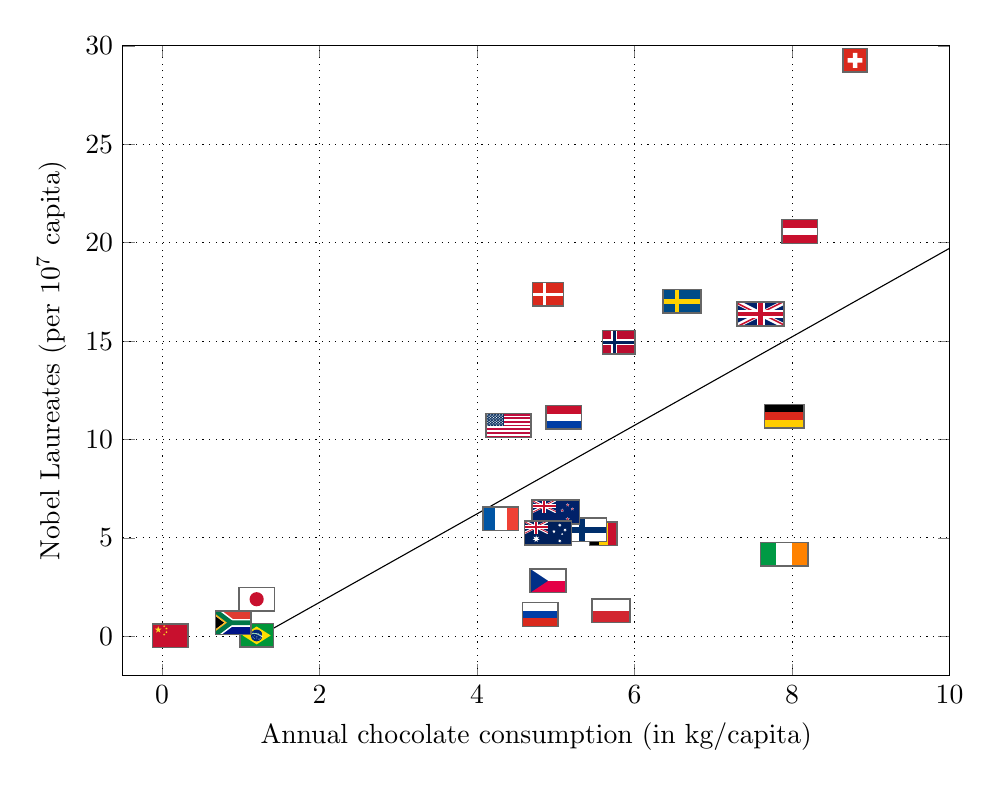
\begin{tikzpicture}[x=10mm,y=2.5mm]
  % I reproduced the visualization in \citep{Messerli2012}, but made use of newer data from \url{https://www.theobroma-cacao.de/wissen/wirtschaft/international/konsum} on chocolate consumption in 2017, and from \url{https://en.wikipedia.org/wiki/List_of_countries_by_Nobel_laureates_per_capita} on scientific Nobel laureates until 2019.
\begin{scope}[xshift=-5mm,yshift=-5mm]
  \begin{axis}[xtick={0,2,4,6,8,10},
  ytick={0,5,10,15,20,25,30},
  xlabel={Annual chocolate consumption (in kg/capita)},
  ylabel={Nobel Laureates (per $10^7$ capita)},
  xlabel style={below},
  ylabel style={above},
  xmin=-0.5,
  xmax=10,
  ymin=-2,
  ymax=30,
  x=10mm,
  y=2.5mm]
  \end{axis}
\end{scope}
  \draw [thin,dotted] (-0.5,0) -- (10,0);
  \draw [thin,dotted] (-0.5,5) -- (10,5);
  \draw [thin,dotted] (-0.5,10) -- (10,10);
  \draw [thin,dotted] (-0.5,15) -- (10,15);
  \draw [thin,dotted] (-0.5,20) -- (10,20);
  \draw [thin,dotted] (-0.5,25) -- (10,25);
  \draw [thin,dotted] (0,-2) -- (0,30);
  \draw [thin,dotted] (2,-2) -- (2,30);
  \draw [thin,dotted] (4,-2) -- (4,30);
  \draw [thin,dotted] (6,-2) -- (6,30);
  \draw [thin,dotted] (8,-2) -- (8,30);
  \draw (1.23,0) -- (10,19.714);
%  \node at (1,24) {$R = 0.69$};
%  \node at (1,25) {$p = 0.0004$};
  \pic (CH) [country=CH,width=3mm] at (8.8,29.260) {worldflag}; % Switzerland
  \pic (AT) [country=AT,width=3mm] at (8.1,20.567) {worldflag}; % Austria
  \pic (DE) [country=DE,width=3mm] at (7.9,11.180) {worldflag}; %Germany
  \pic (IE) [country=IE,width=3mm] at (7.9,4.163) {worldflag}; %Ireland
  \pic (GB) [country=GB,width=3mm] at (7.6,16.373) {worldflag}; %United Kingdom
  \pic (SE) [country=SE,width=3mm] at (6.6,17.029) {worldflag}; %Sweden
  \pic (NO) [country=NO,width=3mm] at (5.8,14.944) {worldflag}; %Norway
  \pic (PL) [country=PL,width=3mm] at (5.7,1.312) {worldflag}; %Poland
  \pic (BE) [country=BE,width=3mm] at (5.6,5.218) {worldflag}; %Belgium
  \pic (FI) [country=FI,width=3mm] at (5.4,5.413) {worldflag}; %Finland
  \pic (NZ) [country=NZ,width=3mm] at (5,6.316) {worldflag}; %New Zealand
  \pic (DK) [country=DK,width=3mm] at (4.9,17.378) {worldflag}; %Denmark
  \pic (AU) [country=AU,width=3mm] at (4.9,5.249) {worldflag}; %Australia
  \pic (CZ) [country=CZ,width=3mm] at (4.9,2.823) {worldflag}; %Czech Republic
  \pic (RU) [country=RU,width=3mm] at (4.8,1.111) {worldflag}; %Russia
  \pic (US) [country=US,width=3mm] at (4.4,10.711) {worldflag}; %USA
  \pic (FR) [country=FR,width=3mm] at (4.3,5.979) {worldflag}; %France
  \pic (BR) [country=BR,width=3mm] at (1.2,0.047) {worldflag}; %Brazil
  \pic (JP) [country=JP,width=3mm] at (1.2,1.887) {worldflag}; %Japan
  \pic (ZA) [country=ZA,width=3mm] at (0.9,0.697) {worldflag}; %South Africa
  \pic (CN) [country=CN,width=3mm] at (0.1,0.035) {worldflag}; %China
%  \draw [line width=1mm,->,red] (5.1,11.12) to (7.65,16.85);
%  \node at (7.65,17.85) {\color{red}$H_1$};
%  \draw [line width=1mm,->,blue] (5.1,11.12) to (7.65,11.12);
%  \node at (7.25,10.12) {\color{blue}$H_2$};
  \pic (NL) [country=NL,width=3mm] at (5.1,11.121) {worldflag}; %Netherlands
\end{tikzpicture}

\end{document}
